% \documentclass[twoside]{article}

% \usepackage{aistats2025}

% If your paper is accepted, change the options for the package
% aistats2025 as follows:
%
%\usepackage[accepted]{aistats2025}
%
% This option will print headings for the title of your paper and
% headings for the authors names, plus a copyright note at the end of
% the first column of the first page.

% If you set papersize explicitly, activate the following three lines:
%\special{papersize = 8.5in, 11in}
%\setlength{\pdfpageheight}{11in}
%\setlength{\pdfpagewidth}{8.5in}

% If you use natbib package, activate the following three lines:
%\usepackage[round]{natbib}
%\renewcommand{\bibname}{References}
%\renewcommand{\bibsection}{\subsubsection*{\bibname}}

% If you use BibTeX in apalike style, activate the following line:
%\bibliographystyle{apalike}

% \begin{document}

% If your paper is accepted and the title of your paper is very long,
% the style will print as headings an error message. Use the following
% command to supply a shorter title of your paper so that it can be
% used as headings.
%
%\runningtitle{I use this title instead because the last one was very long}

% If your paper is accepted and the number of authors is large, the
% style will print as headings an error message. Use the following
% command to supply a shorter version of the authors names so that
% they can be used as headings (for example, use only the surnames)
%
%\runningauthor{Surname 1, Surname 2, Surname 3, ...., Surname n}

% Supplementary material: To improve readability, you must use a single-column format for the supplementary material.
\onecolumn
\aistatstitle{
Trustworthy assessment of heterogeneous treatment effect estimator via analysis of relative error:
Supplementary Materials}
% \vspace{-50pt}

\noindent \textbf{Notations}.
For a causal estimand $\phi$, we use $\IFC(\phi)$ to denote an influence function of $\phi$.
We derive the influence functions assuming the covariates are discrete as in \cite{kennedy2022semiparametric}.
We use $\PP_n$ to denote the distribution of $n$ test data points, and $\EE_n$ be the corresponding expectation (the average over $n$ test data points).

    
% \subsection{PROOFS}\label{appe:sec:proof}

\textbf{A. PROOFS}

\textit{Proof of Theorem 1}. 
    We first derive the efficient influence function for the absolute error~\eqref{defi:evaluation.error}. 
    We next prove the asymptotic distribution of the absolute error estimator~\eqref{eq:estimator.absolute.error}.

    
    \noindent \textbf{Derivation of the efficient influence function}. 
    We consider non-parametric models, where the tangent space contains the entire Hilbert space of mean-zero, finite-variance functions \parencite{tsiatis2006semiparametric}.
    In this case, the influence function is unique, and it must be efficient.
    Below we derive this influence function by applying differentiation rules and using putative influence functions for common causal estimands \parencite{kennedy2022semiparametric}.

    
    By the linearity of influence functions, 
    \begin{align*}
        \IFC(\phi(\hat{\tau}))
        = \underbrace{\IFC\left(\EE\left[\hat{\tau}^2(X_i)\right]\right)}_{:=\text{(a)}} 
        - 2\underbrace{\IFC\left(\EE\left[\hat{\tau}(X_i) {\tau}(X_i)\right]\right)}_{:=\text{(b)}}
        + \underbrace{\IFC\left(\EE\left[\tau^2(X_i)\right]\right)}_{:=\text{(c)}}.
    \end{align*}
    We deal with (a) to (c) one by one.
    For (a), $\hat{\tau}(x)$ is a known function of the covariates, and
    \begin{align}\label{proof:absolute.error.(a)}
        \text{(a)} = \hat{\tau}^2(X_i) - \EE[\hat{\tau}^2(X_i)].
    \end{align}
    For (b), $\EE\left[\hat{\tau}(X_i) {\tau}(X_i)\right]$ is a weighted average treatment effect with weights $\hat{\tau}(X_i)$, and 
    \begin{align}\label{proof:absolute.error.(b)}
        \text{(b)} = \hat{\tau}(X_i) \cdot \left(\frac{W_i(Y_i - \mu_1(X_i))}{e(X_i)} + \mu_1(X_i) - \frac{(1-W_i)(Y_i - \mu_0(X_i))}{1-e(X_i)} - \mu_0(X_i) \right) - \EE[\hat{\tau}(X_i) \tau(X_i)].
    \end{align}
    For (c), we rewrite the second moment as a finite sum, and
    \begin{align}\label{proof:absolute.error.(c)}
        \begin{split}
    \text{(c)} 
        &= \sum_x \IFC(\tau^2(x)) \PP_X(dx) +  \sum_x \tau^2(x) \IFC(\PP_X(dx)) \quad (\text{Linearity, product rule of influence functions})\\
        &= \sum_x 2 \tau(x) \IFC(\tau(x)) \PP_X(dx) + \sum_x \tau^2(x) \IFC(\PP_X(dx)) \quad (\text{Chain rule of influence functions}) \\
        &= 2(\mu_1(X_i) - \mu_0(X_i)) \left(\frac{W_i(Y_i - \mu_1(X_i))}{e(X_i)} - \frac{(1-W_i)(Y_i - \mu_0(X_i))}{1-e(X_i)}\right) \\
        &\quad~ + (\mu_1(X_i) - \mu_0(X_i))^2- \EE[\tau^2(X_i)]. \quad (\text{Influence function of $\tau(x)$, $\PP_X(dx)$.})
        \end{split}
    \end{align}
    Finally, combing (a) to (c) and we have finished the derivation of the influence function for the absolute error~\eqref{defi:evaluation.error}.
       
    \noindent \textbf{Asymptotic distribution of the one-step correction estimator}.
    As in \cite{kennedy2022semiparametric}, we decompose the error into three terms,    
    \begin{align*}
    \hat{\phi}(\hat{\tau}) - {\phi}(\hat{\tau})
        &= \underbrace{\EE_n[{\psi}(\phi(\hat{\tau}); Z_i)] - \EE[{\psi}(\phi(\hat{\tau}); Z_i)]}_{:=\text{S}}  + \underbrace{{\phi}(\hat{\tau}) - \tilde{\phi}(\hat{\tau}) + \EE[\hat{\psi}(\hat{\tau}; Z_i)]}_{:=R} \\
        &\quad~+ \underbrace{\EE_n[\hat{\psi}(\phi(\hat{\tau}); Z_i) - {\psi}(\phi(\hat{\tau}); Z_i)] - \EE[\hat{\psi}(\phi(\hat{\tau}); Z_i) - {\psi}(\phi(\hat{\tau}); Z_i)]}_{:=N},
    \end{align*}
    where $\tilde{\phi}(\hat{\tau})$ denote the absolute error regarding the estimated nuisance functions.
    We deal with $S$, $N$, $R$ one by one.
    For $S$, the U-statistic term, by the central limit theorem, 
    \begin{align}\label{proof:absolute.error.S}
        \begin{split}
            \sqrt{n} S \stackrel{d}{\to} \calN(0, V(\hat{\phi}(\hat{\tau}))).
        \end{split}
    \end{align}
    For $N$, the empirical process term, by the boundedness assumption ($Y_i$ is bounded, $e(X_i)$ is bounded away from zero and one, and the nuisance function estimators $\hat{\mu}_0(x)$, $\hat{\mu}_1(x)$ are bounded, $\hat{e}(x)$ is bounded away from zero and one), and that nuisance function estimators are consistent,
    %TODO: add assumptions of the estimated nuisance functions: and the nuisance function estimators $\hat{\mu}_0(x)$, $\hat{\mu}_1(x)$ are bounded, $\hat{e}(x)$ is bounded away from zero and one,
    \begin{align}\label{proof:absolute.error.N}
        n \var(N)
        = \var\left(\hat{\psi}(\phi(\hat{\tau}); Z_i) - {\psi}(\phi(\hat{\tau}); Z_i)\right)
        \to 0.
    \end{align}
    By Chebyshev's inequality, we have $\sqrt{n}N \stackrel{p}{\to} 0$.
    For $R$, the remainder term, we decompose it into the remainder term of (a), (b), and (c) in \eqref{proof:absolute.error.(a)}, \eqref{proof:absolute.error.(b)}, and \eqref{proof:absolute.error.(c)}, respectively.
    $R$(a) is exactly zero. 
    $R$(b) is the remainder term of a weighted average treatment effect, and satisfies $o_p(n^{-1/2})$ under the boundedness assumption and the assumption that $\hat{\mu}_1(x)$, $\hat{\mu}_0(x)$, and $\hat{e}_1(x)$ converge at rate $o_p(n^{-1/4})$ in $L_2$ norm.
    For $R$(c),
    \begin{align}\label{proof:absolute.error.R}
        \begin{split}
          R\text{(c)}
          &= -\EE\left[((\mu_1(X_i) - \mu_0(X_i)) - (\tilde{\mu}_1(X_i) - \tilde{\mu}_0(X_i)))^2\right] + 2 \EE\left[(\tilde{\mu}_1(X_i) - \tilde{\mu}_0(X_i)) r(X_i)\right], \\
          &\quad~r(x) := \left( \frac{e(x)}{\tilde{e}(x)} - 1 \right) \left( \mu_1(x) - \tilde{\mu}_1(x) \right) 
          - \left( \frac{1 - e(x)}{1 - \tilde{e}(x)} - 1 \right) \left( \mu_0(x) - \tilde{\mu}_0(x) \right).
        \end{split}
    \end{align}
    % TODO: to check R(c).
    Again we use the boundedness assumption, and the $o_p(n^{-1/4})$ convergence assumption of $\tilde{\mu}_1(x)$, $\tilde{\mu}_0(x)$, and $\tilde{e}(x)$,
    \begin{align*}
        \EE\left[|r(X_i)|\right]
        &\le \EE \left[\left
        |\left(\frac{1 - e(X_i)}{1 - \tilde{e}(X_i)} - 1 \right) \left( \mu_0(X_i) - \tilde{\mu}_0(X_i) \right)\right|\right]
        + \EE\left[\left| \left(\frac{1 - e(X_i)}{1 - \tilde{e}(X_i)} - 1 \right) \left( \mu_0(X_i) - \tilde{\mu}_0(X_i) \right)\right|\right]\\
        &\le \EE^{1/2} \left[\left
        (\frac{1 - e(X_i)}{1 - \tilde{e}(X_i)} - 1 \right)^2 \right]  \EE^{1/2} \left[\left( \mu_0(X_i) - \tilde{\mu}_0(X_i) \right)^2\right]\\
        &\quad~+  \EE^{1/2}\left[\left( \frac{1 - e(X_i)}{1 - \tilde{e}(X_i)} - 1 \right)^2\right] \EE^{1/2} \left[ \left( \mu_0(X_i) - \tilde{\mu}_0(X_i) \right)^2\right]
        = o_p(n^{-1/2}).
    \end{align*}
    By the boundedness assumption, there exists $C > 0$ such that
    \begin{align*}
        \EE\left[\left|(\tilde{\mu}_1(X_i) - \tilde{\mu}_0(X_i)) r(X_i)\right|\right]
        &\le C \cdot \EE\left[|r(X_i)|\right] 
        = o_p(n^{-1/2}).
    \end{align*}
    Combining $S$, $N$, $R$ and we have proved $\sqrt{n}(\hat{\phi}(\hat{\tau}) - {\phi}(\hat{\tau})) \stackrel{d}{\to} \calN(0, {V}(\hat{\phi}(\hat{\tau})))$.
    The above derivation considers pre-fixed nuisance function estimators. As for cross-fitting in \Cref{algo:absolute.error}, we apply the argument in \cite{chernozhukov2018double}.
    

    For the variance estimator, by the boundedness assumption and the law of large number,
    \begin{align*}
        \hat{V}(\hat{\phi}(\hat{\tau})) \stackrel{p}{\to} {V}(\hat{\phi}(\hat{\tau})).
    \end{align*}
    By the assumption that $\PP(\hat{\tau}(X_i) \neq {\tau}(X_i)) > 0$, we have ${V}(\hat{\phi}(\hat{\tau})) > 0$.
    Finally, by Slutsky's lemma, we have finished the proof of \Cref{theo:absolute.error}.
    



\begin{proof}[Proof of \Cref{theo:relative.error}]
    Similar to the proof of \Cref{theo:absolute.error},  we first derive the efficient influence function for the relative error~\eqref{defi:evaluation.error.relative}. 
    We next prove the asymptotic distribution of the absolute error estimator~\eqref{eq:estimator.relative.error}.

    \noindent \textbf{Derivation of the efficient influence function}.
    Note that $\delta(\hat{\tau}_1, \hat{\tau}_2) = \phi(\hat{\tau}_1) - \phi(\hat{\tau}_2)$. By the linearity of influence functions, the influence function for $\delta(\hat{\tau}_1, \hat{\tau}_2)$ is simply the difference between the influence function of $\phi(\hat{\tau}_1)$ and that of $\phi(\hat{\tau}_2)$ derived in \Cref{theo:absolute.error}. 
    Alternatively, recognize that the estimand $\delta(\hat{\tau}_1, \hat{\tau}_2)$ is a weighted average treatment effect, for which the influence function is a well-established result.
    Both methods lead to the influence function~\eqref{eq:EIF.relative}.


    \noindent \textbf{Asymptotic distribution of the one-step correction estimator}.
    Given that the estimand $\delta(\hat{\tau}_1, \hat{\tau}_2)$ is a weighted average treatment effect, the asymptotic distribution of the one-step correction estimator, under the assumptions of \Cref{theo:relative.error}, follows from the standard result \parencite{kennedy2022semiparametric}. 
    Regarding cross-fitting, we apply the analysis in \cite{chernozhukov2018double}. 
    % TODO: add the boundedness assumption.
    
    Additionally, the degeneracy assumption $\mathbb{P}(\hat{\tau}_1(X_i) \neq \hat{\tau}_2(X_i)) > 0$ is required to ensure that the one-step correction estimator, when scaled by $\sqrt{n}$, has a non-zero variance. 
    This also arises in the proof of \Cref{theo:absolute.error}.
\end{proof}


\begin{proposition}\label{prop:relative.error.CI.width}
    There exists $C > 0$ such that
    \begin{align*}
        V(\hat{\delta}(\hat{\tau}_1, \hat{\tau}_2)) \le C \cdot \EE[(\hat{\tau}_1(X) - \hat{\tau}_2(X))^2].
    \end{align*}
    This together with \Cref{theo:relative.error} implies the width of the confidence interval of the relative error estimator~\eqref{eq:estimator.relative.error} based on \Cref{theo:relative.error} is of order $\sqrt{\EE[(\hat{\tau}_1(X) - \hat{\tau}_2(X))^2]} \cdot {n}^{-1/2}$.
\end{proposition}


\begin{proof}[Proof of \Cref{prop:relative.error.CI.width}]
    By Cauchy-Schwarz inequality, 
    \begin{align*}
        V(\hat{\delta}(\hat{\tau}_1, \hat{\tau}_2))
        &\le \EE\left[(\hat{\tau}_2(X_i) - \hat{\tau}_1(X_i))^2\right] \cdot \EE\left[\left(\frac{W_i(Y_i - {\mu}_1(X_i))}{{e}(X_i)} + {\mu}_1(X_i) - \frac{(1-W_i)(Y_i - {\mu}_0(X_i))}{1-{e}(X_i)} - {\mu}_0(X_i)\right)^2\right] \\
        &\le C \cdot \EE\left[(\hat{\tau}_2(X_i) - \hat{\tau}_1(X_i))^2\right].  \quad (\text{Boundedness assumption})
    \end{align*}
\end{proof}


\begin{corollary}[DINA]\label{prop:DINA}
    \Cref{theo:absolute.error}, \Cref{theo:relative.error} hold for the causal estimands in \Cref{rmk:DINA}.
\end{corollary}

\begin{proof}[Proof of \label{prop:DINA}]

    To derive the influence functions for the causal estimand in \Cref{rmk:DINA}, we can apply the chain rule of influence functions to the proofs of \Cref{theo:absolute.error}, \Cref{theo:relative.error}.

    For the asymptotic distribution of the one-step correction estimator, we can still apply the arguments in \Cref{theo:absolute.error} and \Cref{theo:relative.error}.
\end{proof}

% previous
% \begin{proof}[Proof of \Cref{prop:relative.error.CI.width}]
% \begin{align*}
%     &\frac{\hat{\delta}(\hat{\tau}_1, \hat{\tau}_2) - {\delta}(\hat{\tau}_1, \hat{\tau}_2)}{\sqrt{\frac{1}{n}\sum_{i=1}^n (\hat{\tau}_1(X_i) - \hat{\tau}_2(X_i))^2}} \\
%     &= \frac{1}{n} \sum_{i=1}^n \frac{\hat{\tau}_1(X_i) - \hat{\tau}_2(X_i)}{\sqrt{\EE[(\hat{\tau}_1(X) - \hat{\tau}_2(X))^2]}} \left(\hat{\tau}_1(X_i) + \hat{\tau}_2(X_i) + \frac{2W_i(Y_i - \tilde{\mu}_1^{-k}(X_i))}{\tilde{e}^{-k}(X_i)} + 2\tilde{\mu}_1^{-k}(X_i) - \frac{2(1-W_i)(Y_i - \tilde{\mu}_0^{-k}(X_i))}{1-\tilde{e}^{-k}(X_i)} - 2\tilde{\mu}_0^{-k}(X_i) \right) \\
%     &- \frac{{\delta}(\hat{\tau}_1, \hat{\tau}_2)}{\sqrt{\EE[(\hat{\tau}_1(X) - \hat{\tau}_2(X))^2]}}\\
%     &= \underbrace{\frac{1}{n} \sum_{i=1}^n \frac{\hat{\tau}_1(X_i) - \hat{\tau}_2(X_i)}{\sqrt{\EE[(\hat{\tau}_1(X) - \hat{\tau}_2(X))^2]}} \left(\hat{\tau}_1(X_i) + \hat{\tau}_2(X_i) + 2 \tau(X_i) + \frac{2W_i(Y_i - {\mu}_1(X_i))}{{e}(X_i)} - \frac{(1-W_i)(Y_i - {\mu}_0(X_i))}{1-{e}(X_i)}\right) - \frac{{\delta}(\hat{\tau}_1, \hat{\tau}_2)}{\sqrt{\EE[(\hat{\tau}_1(X) - \hat{\tau}_2(X))^2]}}}_{:=\text{(a)}} \\
%     & + \frac{2}{n} \sum_{i=1}^n \frac{\hat{\tau}_1(X_i) - \hat{\tau}_2(X_i)}{\sqrt{\EE[(\hat{\tau}_1(X) - \hat{\tau}_2(X))^2]}} \left(\frac{W_i(\mu_1(X_i) - \tilde{\mu}_1^{-k}(X_i))}{\tilde{e}^{-k}(X_i)} + \tilde{\mu}_1^{-k}(X_i) - \frac{(1-W_i)(Y_i - \tilde{\mu}_0^{-k}(X_i))}{1-\tilde{e}^{-k}(X_i)} - \tilde{\mu}_0^{-k}(X_i) - \tau(X_i)  \right) \\
%     &= \frac{1}{n} \sum_{i=1}^n \frac{\hat{\tau}_1(X_i) - \hat{\tau}_2(X_i)}{\sqrt{\EE[(\hat{\tau}_1(X) - \hat{\tau}_2(X))^2]}} \left(\hat{\tau}_1(X_i) + \hat{\tau}_2(X_i) + 2 \tau(X_i)\right) - \frac{{\delta}(\hat{\tau}_1, \hat{\tau}_2)}{\sqrt{\EE[(\hat{\tau}_1(X) - \hat{\tau}_2(X))^2]}} \\
%     & + \frac{2}{n} \sum_{i=1}^n \frac{\hat{\tau}_1(X_i) - \hat{\tau}_2(X_i)}{\sqrt{\EE[(\hat{\tau}_1(X) - \hat{\tau}_2(X))^2]}} (
%     {W_i(Y_i - {\mu}_1(X_i))}(\frac{1}{\tilde{e}^{-k}(X_i)} - \frac{1}{{e}(X_i)}) \\
%     &+ \frac{(W_i - {e}(X_i))(\tilde{\mu}_1^{-k}(X_i) - \tilde{\mu}_1(X_i))}{\tilde{e}^{-k}(X_i)} + \frac{({e}(X_i) - \tilde{e}^{-k}(X_i))(\tilde{\mu}_1^{-k}(X_i) - \tilde{\mu}_1(X_i))}{\tilde{e}^{-k}(X_i)} ) \\
%     &\stackrel{d}{\to} \calN(0, \frac{V(\delta(\hat{\tau}_1, \hat{\tau}_2))}{\EE[(\hat{\tau}_1(X) - \hat{\tau}_2(X))^2]})
% \end{align*}
% (a) multiplied by $\sqrt{n}$ converges to $\calN(0, \frac{???} {\EE[(\hat{\tau}_1(X) - \hat{\tau}_2(X))^2]})$ by Slutsky and CLT of i.i.d. random variables.
% By Cauchy Swartz, (b) squared is upper bounded by 
% \begin{align*}
%     \frac{1}{n} \sum_{i=1}^n \frac{(\hat{\tau}_1(X_i) - \hat{\tau}_2(X_i))^2}{\EE[(\hat{\tau}_1(X) - \hat{\tau}_2(X))^2]} 
%     \cdot \frac{1}{n} \sum_{i=1}^n \frac{(\hat{\tau}_1(X_i) - \hat{\tau}_2(X_i))^2}{\EE[(\hat{\tau}_1(X) - \hat{\tau}_2(X))^2]}  
% \end{align*}
% \end{proof}




% \section{ADDITIONAL EMPIRICAL EXPERIMENTS}\label{appe:sec:simulation.additional}
\textbf{B ADDITIONAL EMPIRICAL EXPERIMENTS} 

We provide additional demonstrations of the hypothetical real data analysis in \Cref{sec:simulation}. The datasets, HTE estimators, and evaluation methods remain the same. 
In Section B.1, we present the widths of the confidence intervals, which can serve as an indication of the statistical power (shorter confidence interval suggests higher power). 
In Section B.2, we report the estimation errors for both the absolute and relative error estimators, that is $|\hat{\phi}(\hat{\tau}) - \phi(\hat{\tau})|$ and $|\hat{\delta}(\hat{\tau}_1, \hat{\tau}_2) - \delta(\hat{\tau}_1, \hat{\tau}_2)|$.


% \subsection{Widths of confidence intervals}\label{appe:sec:simulation.width}
\textbf{B.1 Widths of confidence intervals}

In \Cref{fig:ACIC.width}, we report the widths of the estimated absolute (LASSO, Boosting) and relative (LASSO vs. Boosting) error 90\% confidence intervals across three methods (plug-in, IF, EIF) over four scenarios from the ACIC competition data ((a) to (d)).
Shorter widths indicate higher power of identifying the better HTE estimator.


We make the following observations:
\begin{itemize}
    \item Across all settings and methods, the confidence intervals for the relative error estimators are significantly shorter than those for the absolute error estimators.
    \item For the absolute error estimators, our proposal (EIF) performs significantly better than the estimator in \cite{alaa2019validating} (IF) in scenario (d), and the two methods are comparable in scenarios (a) to (c). The plug-in estimator (plug in) produces the widest intervals across all settings.
\end{itemize}


\begin{figure}[ht]
        \centering
        \begin{minipage}{0.3\textwidth}
                \centering
                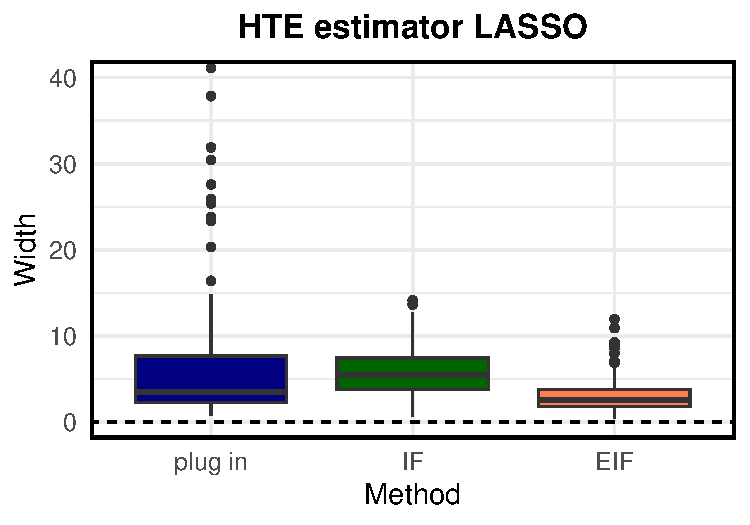
\includegraphics[clip, trim = 0cm 0cm 0cm 0cm, width = \textwidth]{plot/ACIC_linear_propensity_linear_HTE_CI_width_LASSO.pdf}
        \end{minipage}
        \begin{minipage}{0.3\textwidth}
                \centering
                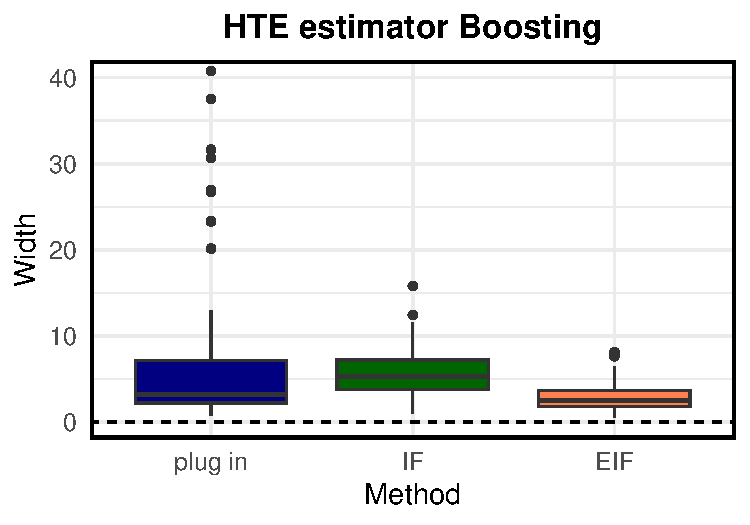
\includegraphics[clip, trim = 0cm 0cm 0cm 0cm, width = \textwidth]{plot/ACIC_linear_propensity_linear_HTE_CI_width_Boosting.pdf}
        \end{minipage}
        \begin{minipage}{0.3\textwidth}
                \centering
                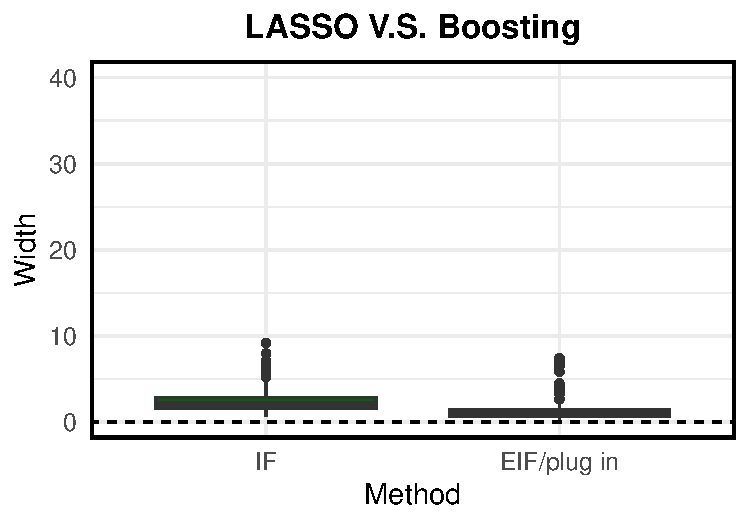
\includegraphics[clip, trim = 0cm 0cm 0cm 0cm, width = \textwidth]{plot/ACIC_linear_propensity_linear_HTE_CI_width_LASSO_V.S._Boosting.pdf}
        \end{minipage}        
        \centering{(a) Linear $\mu_0(x)$, $\mu_1(x)$, linear $e(x)$}\\
        \begin{minipage}{0.3\textwidth}
                \centering
                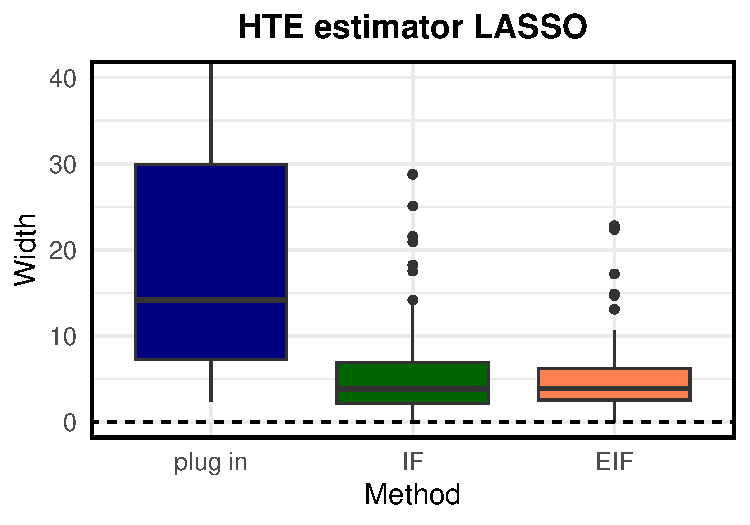
\includegraphics[clip, trim = 0cm 0cm 0cm 0cm, width = \textwidth]{plot/ACIC_linear_propensity_nonlinear_HTE_CI_width_LASSO.pdf}
        \end{minipage}
        \begin{minipage}{0.3\textwidth}
                \centering
                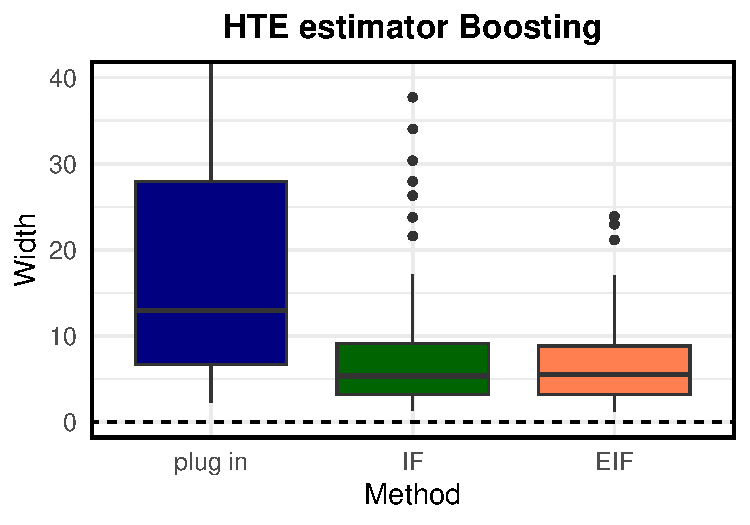
\includegraphics[clip, trim = 0cm 0cm 0cm 0cm, width = \textwidth]{plot/ACIC_linear_propensity_nonlinear_HTE_CI_width_Boosting.pdf}
        \end{minipage}
        \begin{minipage}{0.3\textwidth}
                \centering
                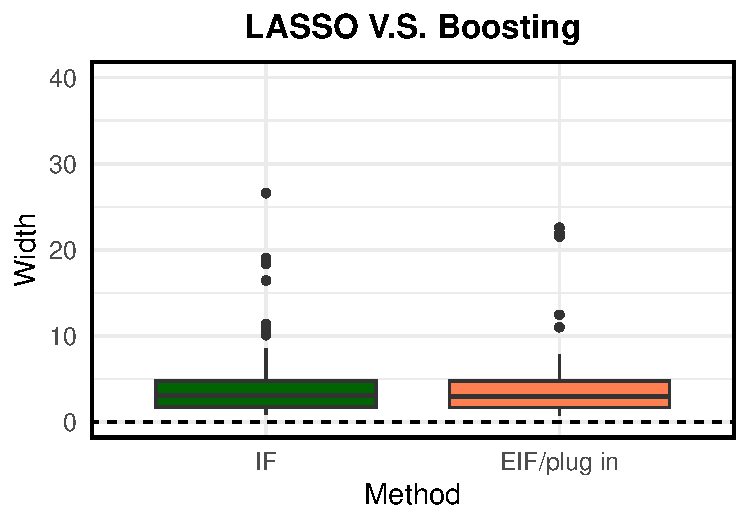
\includegraphics[clip, trim = 0cm 0cm 0cm 0cm, width = \textwidth]{plot/ACIC_linear_propensity_nonlinear_HTE_CI_width_LASSO_V.S._Boosting.pdf}
        \end{minipage}        
        \centering{(b) Nonlinear $\mu_0(x)$, $\mu_1(x)$, linear $e(x)$}  \\        
        \begin{minipage}{0.3\textwidth}
                \centering
                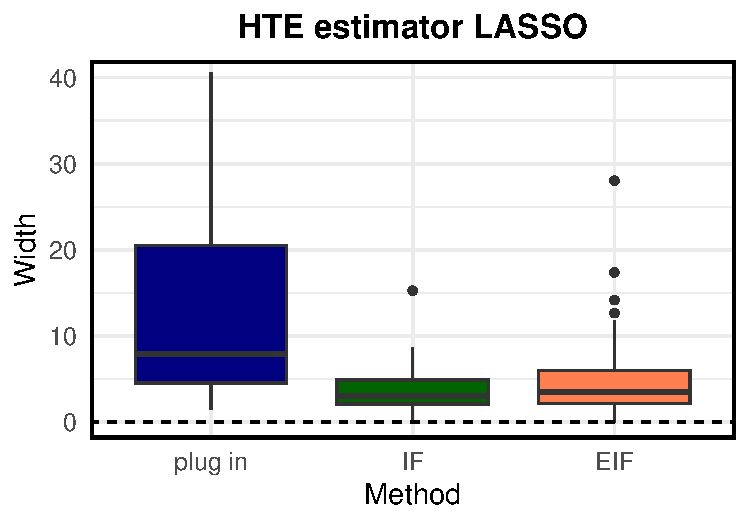
\includegraphics[clip, trim = 0cm 0cm 0cm 0cm, width = \textwidth]{plot/ACIC_nonlinear_propensity_linear_HTE_CI_width_LASSO.pdf}
        \end{minipage}
        \begin{minipage}{0.3\textwidth}
                \centering
                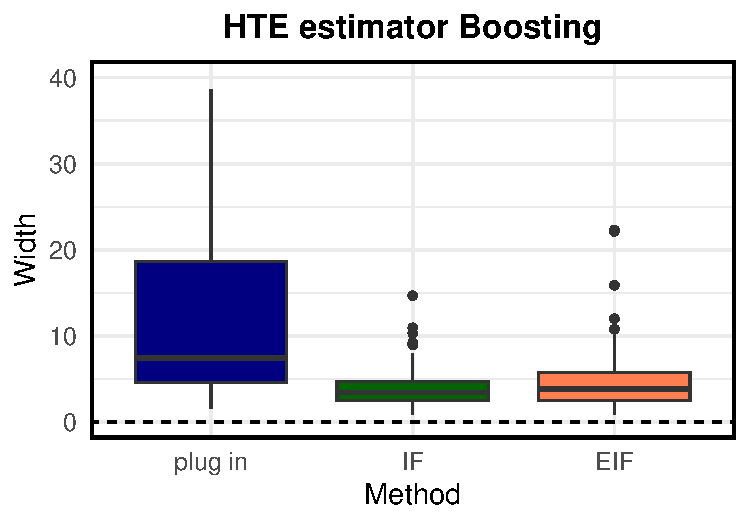
\includegraphics[clip, trim = 0cm 0cm 0cm 0cm, width = \textwidth]{plot/ACIC_nonlinear_propensity_linear_HTE_CI_width_Boosting.pdf}
        \end{minipage}
        \begin{minipage}{0.3\textwidth}
                \centering
                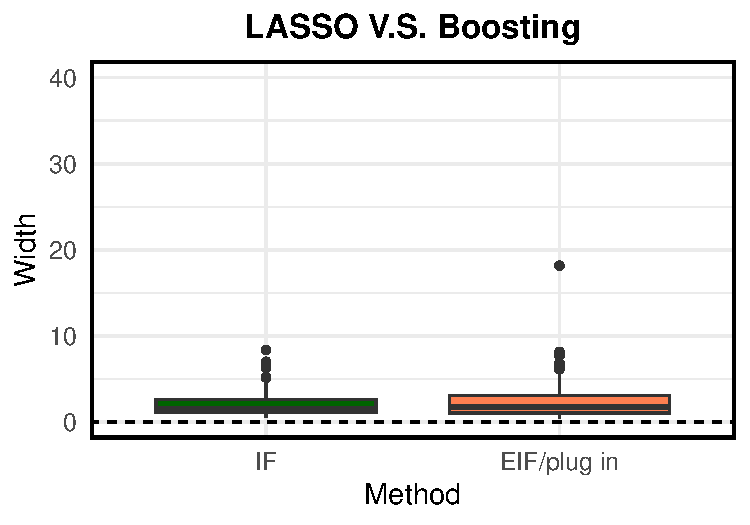
\includegraphics[clip, trim = 0cm 0cm 0cm 0cm, width = \textwidth]{plot/ACIC_nonlinear_propensity_linear_HTE_CI_width_LASSO_V.S._Boosting.pdf}
        \end{minipage}        
        \centering{(c) Linear $\mu_0(x)$, $\mu_1(x)$, nonlinear $e(x)$}    \\  
        \begin{minipage}{0.3\textwidth}
                \centering
                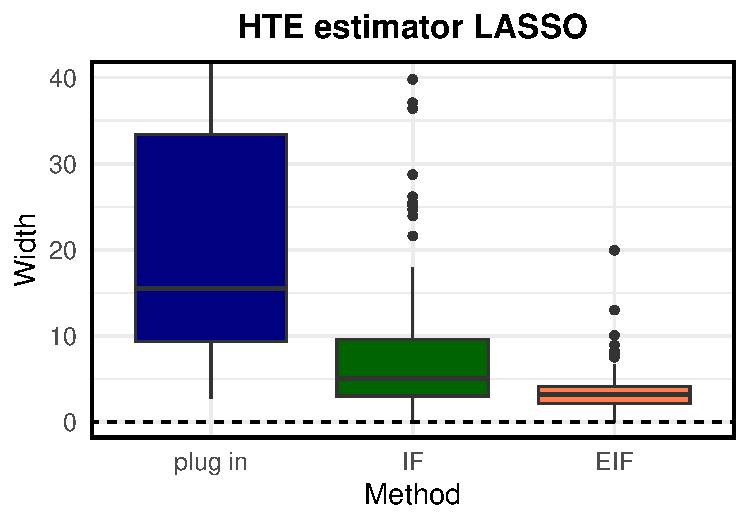
\includegraphics[clip, trim = 0cm 0cm 0cm 0cm, width = \textwidth]{plot/ACIC_nonlinear_propensity_nonlinear_HTE_CI_width_LASSO.pdf}
        \end{minipage}
        \begin{minipage}{0.3\textwidth}
                \centering
                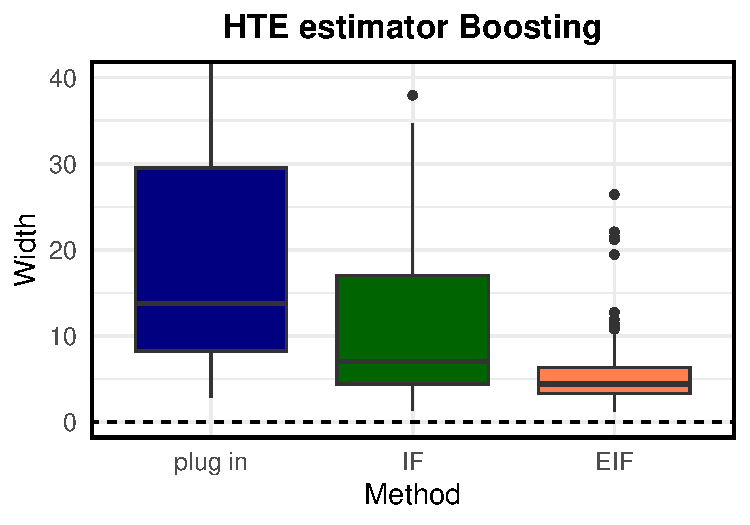
\includegraphics[clip, trim = 0cm 0cm 0cm 0cm, width = \textwidth]{plot/ACIC_nonlinear_propensity_nonlinear_HTE_CI_width_Boosting.pdf}
        \end{minipage}
        \begin{minipage}{0.3\textwidth}
                \centering
                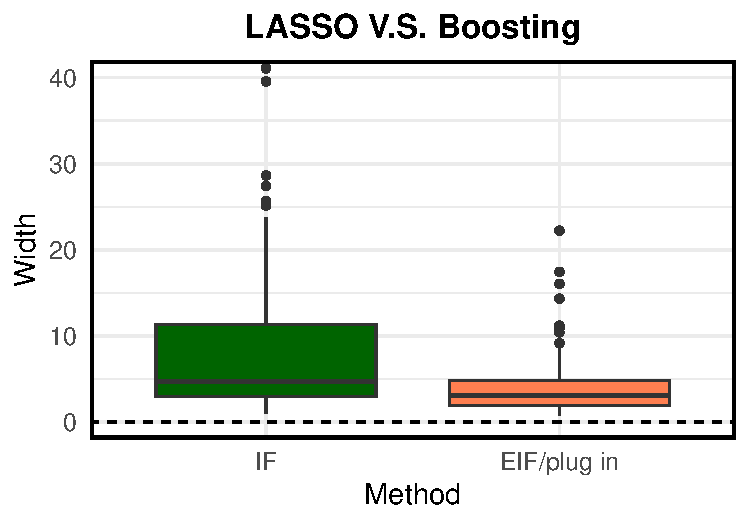
\includegraphics[clip, trim = 0cm 0cm 0cm 0cm, width = \textwidth]{plot/ACIC_nonlinear_propensity_nonlinear_HTE_CI_width_LASSO_V.S._Boosting.pdf}
        \end{minipage}        
        \centering{(d) Nonlinear $\mu_0(x)$, $\mu_1(x)$, nonlinear $e(x)$} \\
        \caption{
        Width of the estimated absolute (LASSO, Boosting)/relative (LASSO V.S. Boosting) error's $90\%$ confidence intervals across three methods (plug in, IF, EIF) over four scenarios of the ACIC competition data ((a) to (d)). 
        }
    \label{fig:ACIC.width}
\end{figure}


% \subsection{Error of estimated errors}\label{appe:sec:simulation.estimation.error}
\textbf{B.2 Error of estimated errors}

In \Cref{fig:ACIC.error.estimated.error}, we report the error of the estimated absolute (LASSO, Boosting)/relative (LASSO V.S. Boosting) error across three methods (plug in, IF, EIF) over four scenarios of the ACIC competition data ((a) to (d)). 
Error of the estimated error is defined as the absolute difference between the estimated error and the corresponding oracle value.
Smaller errors suggest that the estimator has higher accuracy and is thus more favorable.


We make the following observations.
\begin{itemize}
    \item Across all settings and methods, the errors of the relative error estimators are significantly smaller than those for the absolute error estimators.
    \item For the absolute error estimators, our proposal (EIF) performs significantly better than the estimator in \cite{alaa2019validating} (IF) and the plug-in estimator (plug in) in scenario (d). The plug-in estimator is unfavorable from scenarios (b) to (d).
\end{itemize}


\begin{figure}[ht]
          \centering
        \begin{minipage}{0.3\textwidth}
                \centering
                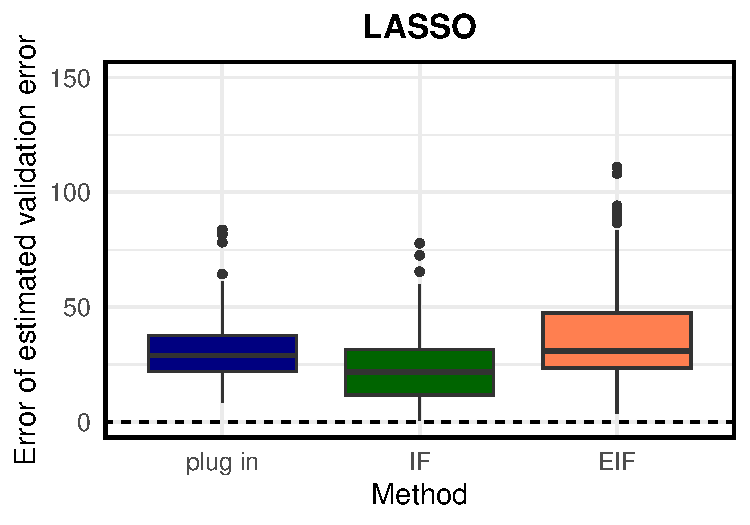
\includegraphics[clip, trim = 0cm 0cm 0cm 0cm, width = \textwidth]{plot/ACIC_linear_propensity_linear_HTE_estimator_error_LASSO.pdf}
        \end{minipage}
        \begin{minipage}{0.3\textwidth}
                \centering
                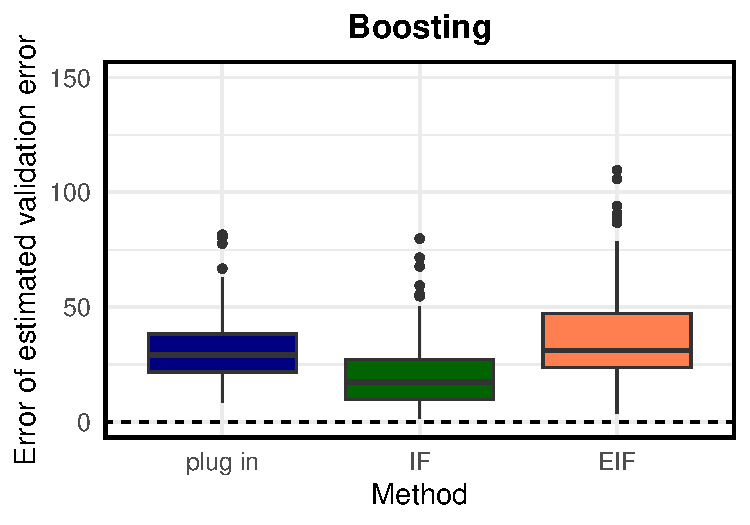
\includegraphics[clip, trim = 0cm 0cm 0cm 0cm, width = \textwidth]{plot/ACIC_linear_propensity_linear_HTE_estimator_error_Boosting.pdf}
        \end{minipage}
        \begin{minipage}{0.3\textwidth}
                \centering
                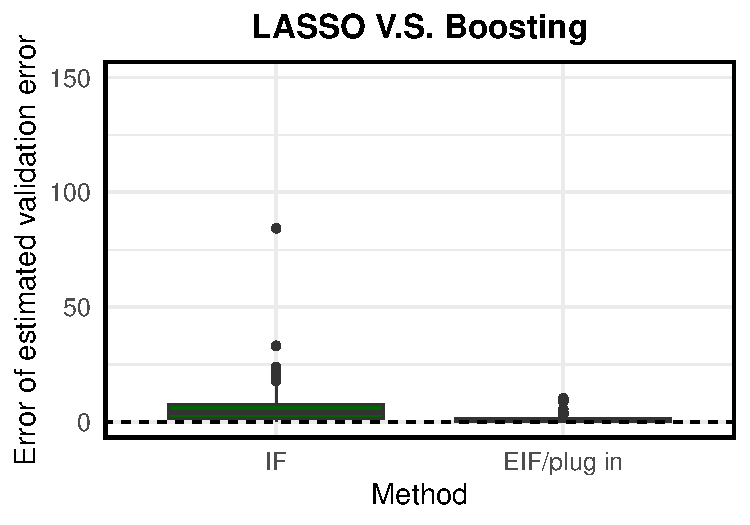
\includegraphics[clip, trim = 0cm 0cm 0cm 0cm, width = \textwidth]{plot/ACIC_linear_propensity_linear_HTE_estimator_error_LASSO_V.S._Boosting.pdf}
        \end{minipage}        
        \centering{(a) Linear $\mu_0(x)$, $\mu_1(x)$, linear $e(x)$}\\
        \begin{minipage}{0.3\textwidth}
                \centering
                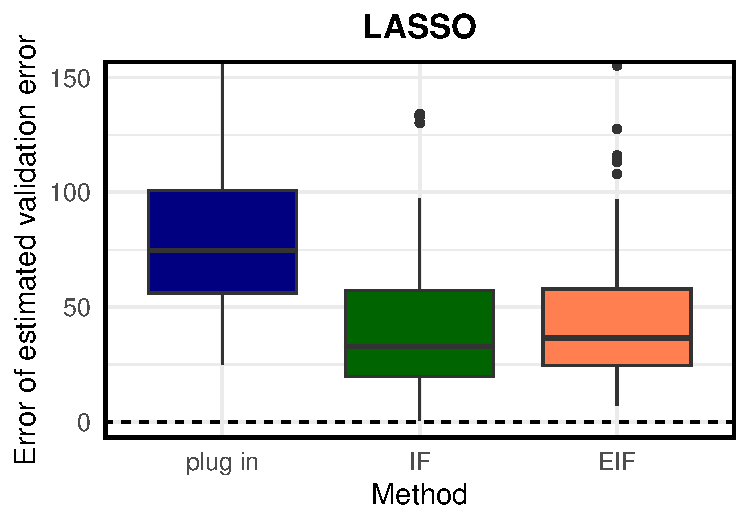
\includegraphics[clip, trim = 0cm 0cm 0cm 0cm, width = \textwidth]{plot/ACIC_linear_propensity_nonlinear_HTE_estimator_error_LASSO.pdf}
        \end{minipage}
        \begin{minipage}{0.3\textwidth}
                \centering
                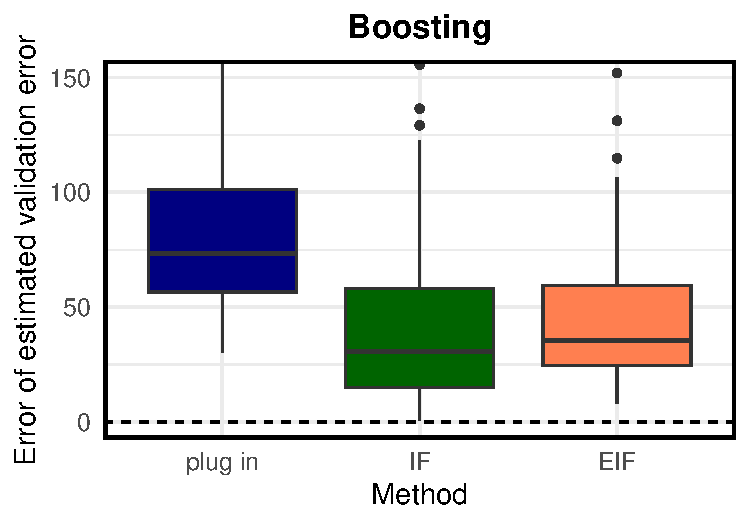
\includegraphics[clip, trim = 0cm 0cm 0cm 0cm, width = \textwidth]{plot/ACIC_linear_propensity_nonlinear_HTE_estimator_error_Boosting.pdf}
        \end{minipage}
        \begin{minipage}{0.3\textwidth}
                \centering
                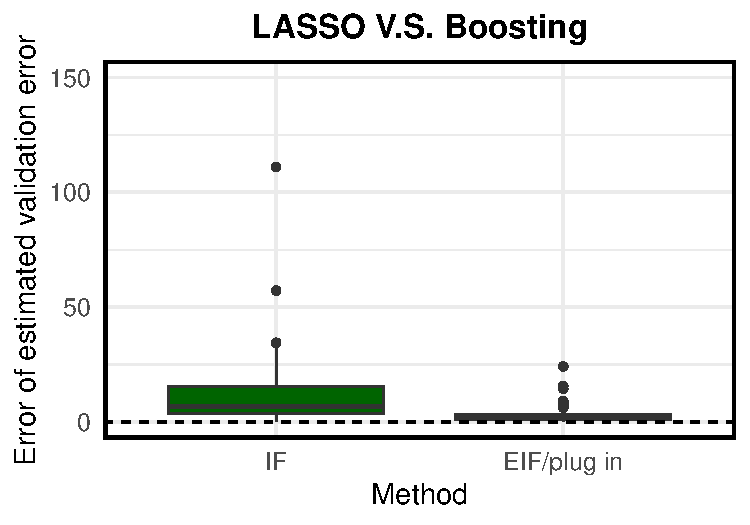
\includegraphics[clip, trim = 0cm 0cm 0cm 0cm, width = \textwidth]{plot/ACIC_linear_propensity_nonlinear_HTE_estimator_error_LASSO_V.S._Boosting.pdf}
        \end{minipage}        
        \centering{(b) Nonlinear $\mu_0(x)$, $\mu_1(x)$, linear $e(x)$}  \\
        \begin{minipage}{0.3\textwidth}
                \centering
                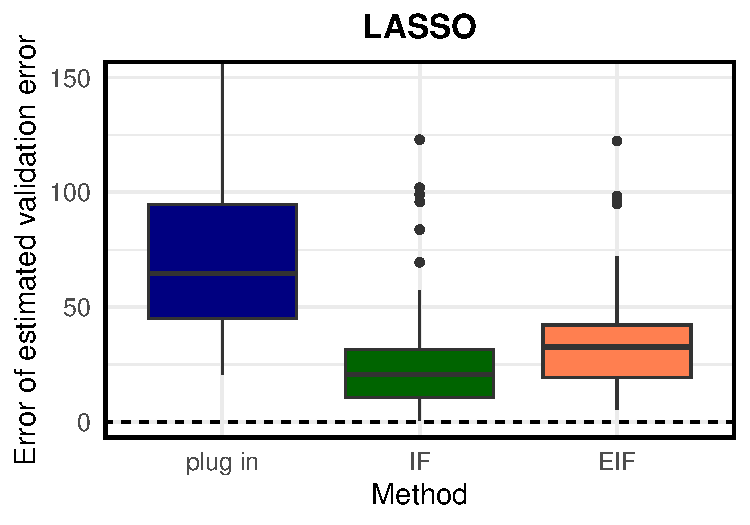
\includegraphics[clip, trim = 0cm 0cm 0cm 0cm, width = \textwidth]{plot/ACIC_nonlinear_propensity_linear_HTE_estimator_error_LASSO.pdf}
        \end{minipage}        
        \begin{minipage}{0.3\textwidth}
                \centering
                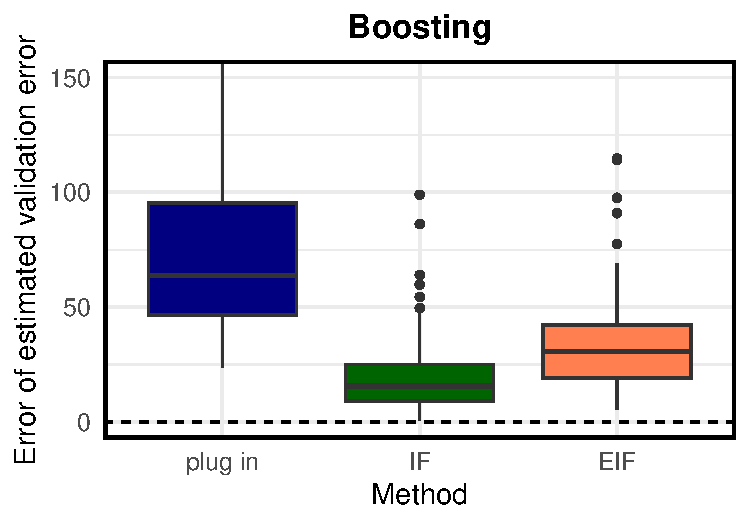
\includegraphics[clip, trim = 0cm 0cm 0cm 0cm, width = \textwidth]{plot/ACIC_nonlinear_propensity_linear_HTE_estimator_error_Boosting.pdf}
        \end{minipage}
        \begin{minipage}{0.3\textwidth}
                \centering
                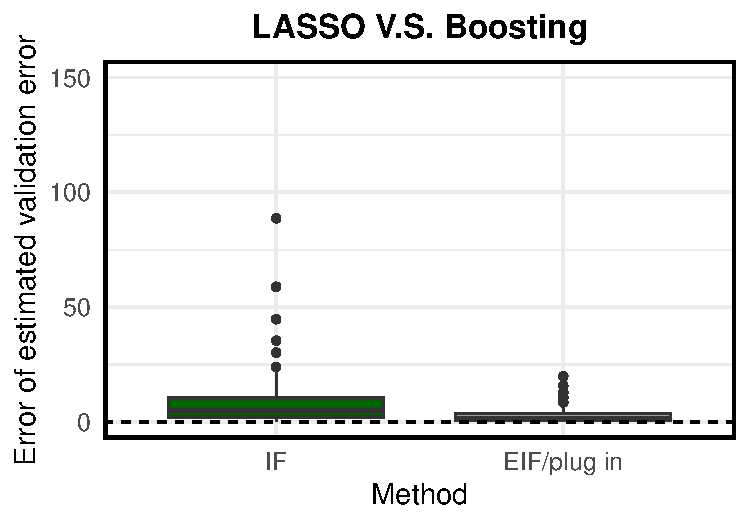
\includegraphics[clip, trim = 0cm 0cm 0cm 0cm, width = \textwidth]{plot/ACIC_nonlinear_propensity_linear_HTE_estimator_error_LASSO_V.S._Boosting.pdf}
        \end{minipage}        
        \centering{(c) Linear $\mu_0(x)$, $\mu_1(x)$, nonlinear $e(x)$}      \\
        \begin{minipage}{0.3\textwidth}
                \centering
                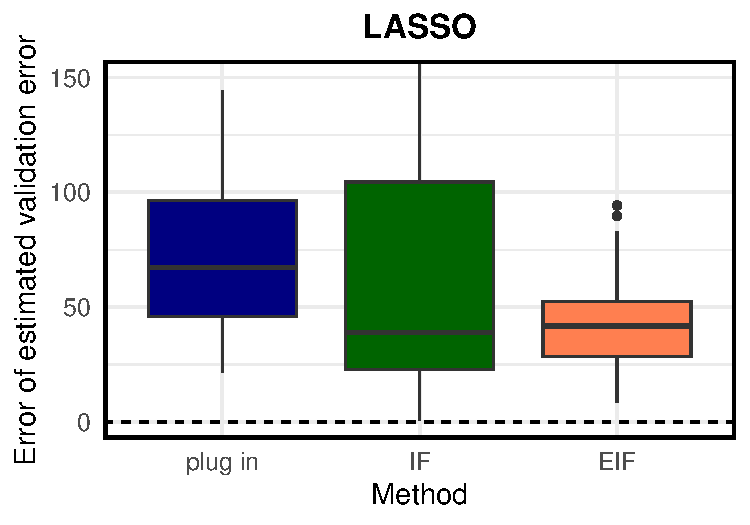
\includegraphics[clip, trim = 0cm 0cm 0cm 0cm, width = \textwidth]{plot/ACIC_nonlinear_propensity_nonlinear_HTE_estimator_error_LASSO.pdf}
        \end{minipage}
        \begin{minipage}{0.3\textwidth}
                \centering
                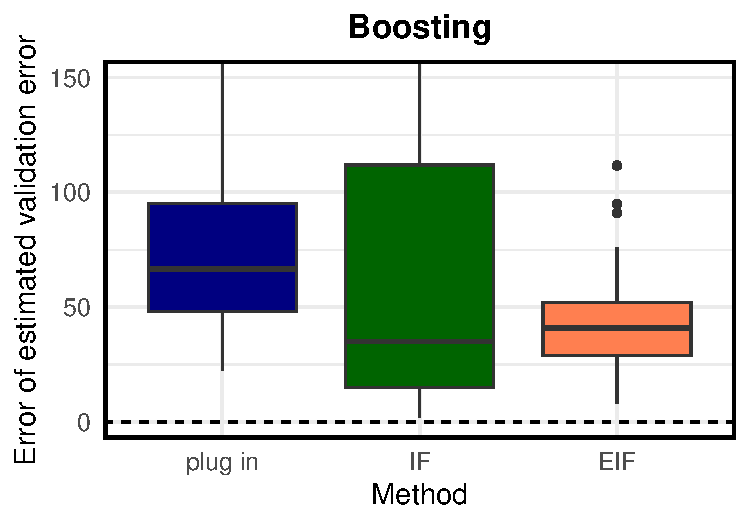
\includegraphics[clip, trim = 0cm 0cm 0cm 0cm, width = \textwidth]{plot/ACIC_nonlinear_propensity_nonlinear_HTE_estimator_error_Boosting.pdf}
        \end{minipage}
        \begin{minipage}{0.3\textwidth}
                \centering
                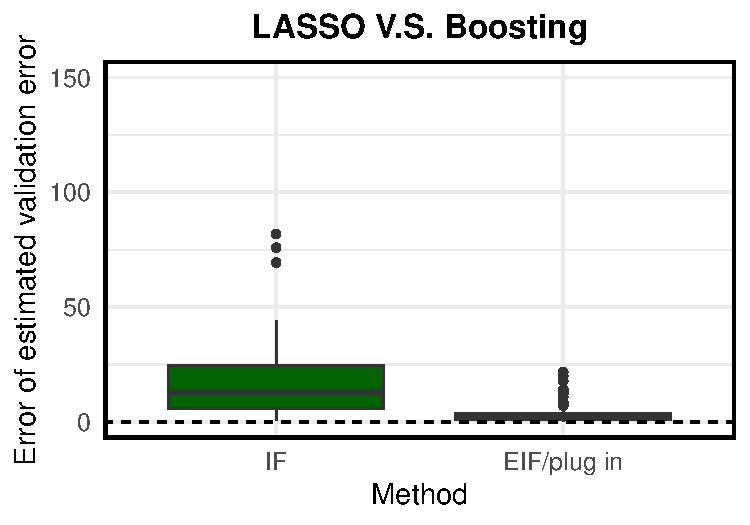
\includegraphics[clip, trim = 0cm 0cm 0cm 0cm, width = \textwidth]{plot/ACIC_nonlinear_propensity_nonlinear_HTE_estimator_error_LASSO_V.S._Boosting.pdf}
        \end{minipage}        
        \centering{(d) Nonlinear $\mu_0(x)$, $\mu_1(x)$, nonlinear $e(x)$} \\
       \caption{
        Error of the estimated absolute (LASSO, Boosting)/relative (LASSO V.S. Boosting) error across three methods (plug in, IF, EIF) over four scenarios of the ACIC competition data ((a) to (d)). 
        Error of the estimated error is defined as the absolute difference between the estimated error and the corresponding oracle value.
        }
    \label{fig:ACIC.error.estimated.error}
\end{figure}





% \begin{figure}[ht]
%         \centering
%         \begin{minipage}{0.3\textwidth}
%                 \centering
%                 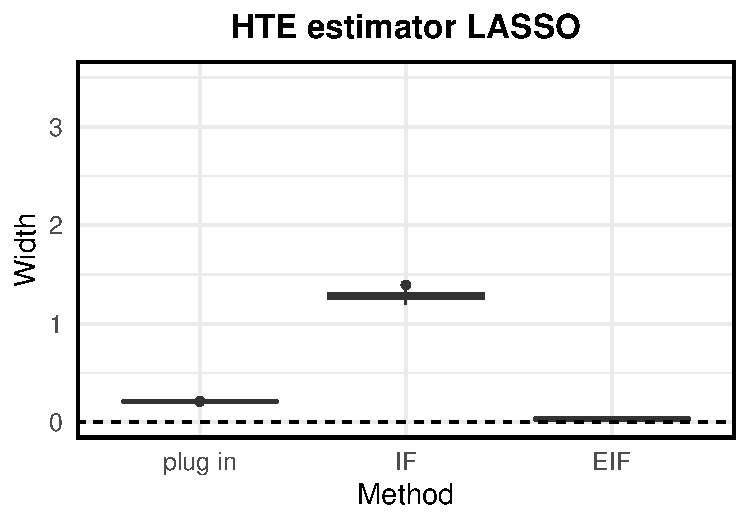
\includegraphics[clip, trim = 0cm 0cm 0cm 0cm, width = \textwidth]{plot/simulation true CI width LASSO.pdf}
%         \end{minipage}
%         \begin{minipage}{0.3\textwidth}
%                 \centering
%                 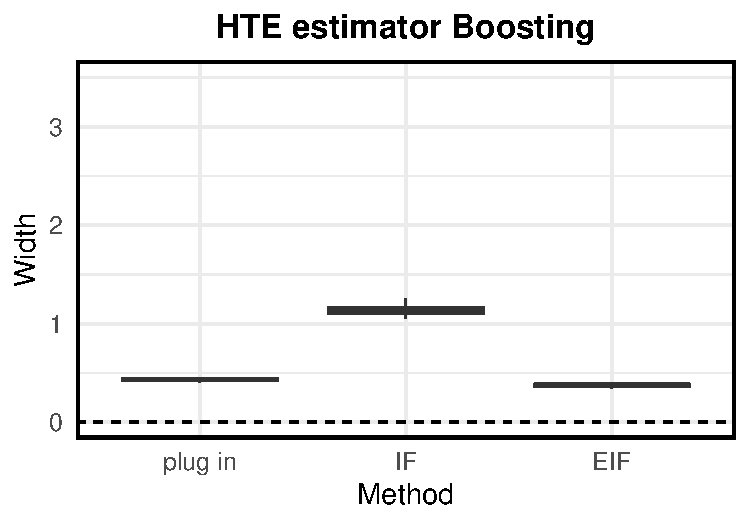
\includegraphics[clip, trim = 0cm 0cm 0cm 0cm, width = \textwidth]{plot/simulation true CI width Boosting.pdf}
%         \end{minipage}
%         \begin{minipage}{0.3\textwidth}
%                 \centering
%                 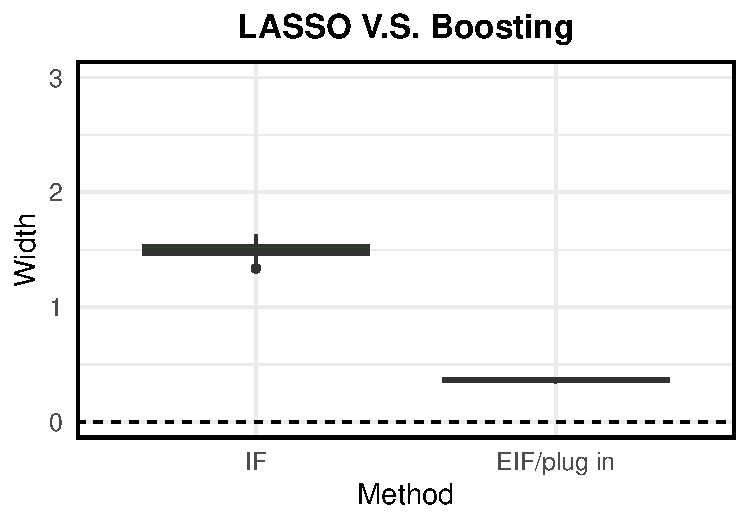
\includegraphics[clip, trim = 0cm 0cm 0cm 0cm, width = \textwidth]{plot/simulation true CI width LASSO V.S. Boosting.pdf}
%         \end{minipage}        
%         \centering{(a) True}          
%         \begin{minipage}{0.3\textwidth}
%                 \centering
%                 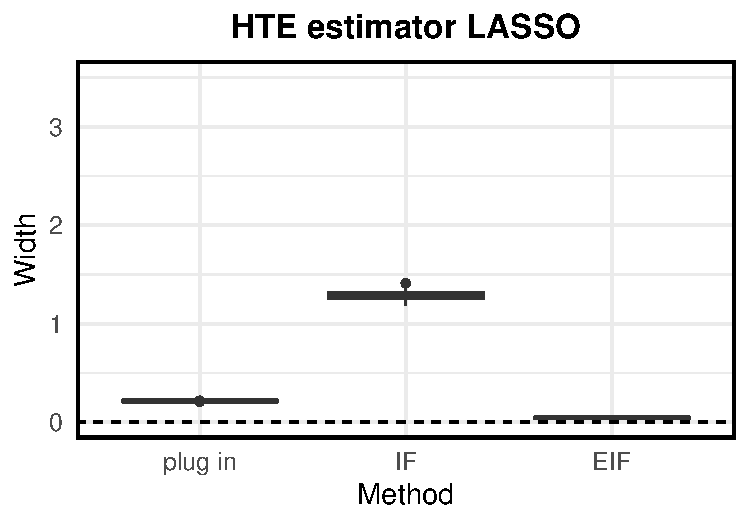
\includegraphics[clip, trim = 0cm 0cm 0cm 0cm, width = \textwidth]{plot/simulation linear CI width LASSO.pdf}
%         \end{minipage}
%         \begin{minipage}{0.3\textwidth}
%                 \centering
%                 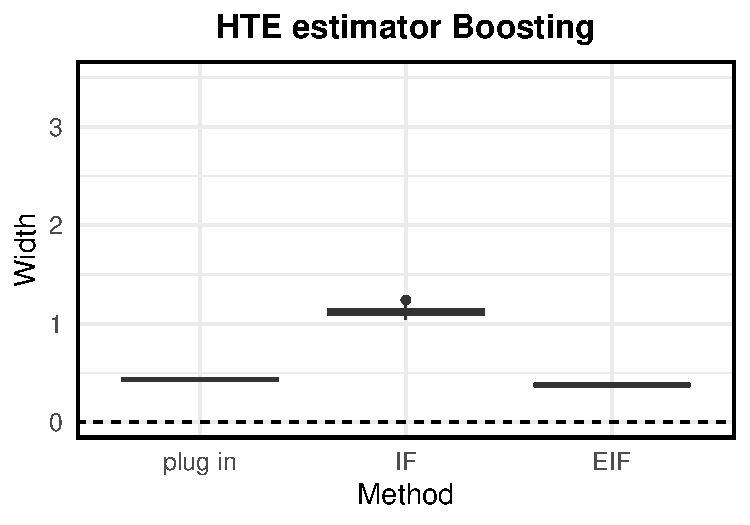
\includegraphics[clip, trim = 0cm 0cm 0cm 0cm, width = \textwidth]{plot/simulation linear CI width Boosting.pdf}
%         \end{minipage}
%         \begin{minipage}{0.3\textwidth}
%                 \centering
%                 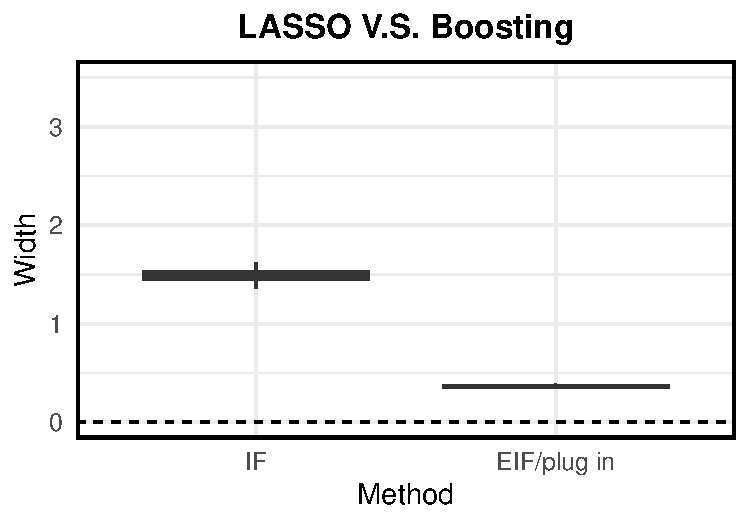
\includegraphics[clip, trim = 0cm 0cm 0cm 0cm, width = \textwidth]{plot/simulation linear CI width LASSO V.S. Boosting.pdf}
%         \end{minipage}        
%         \centering{(b) Linear regression}
%         \begin{minipage}{0.3\textwidth}
%                 \centering
%                 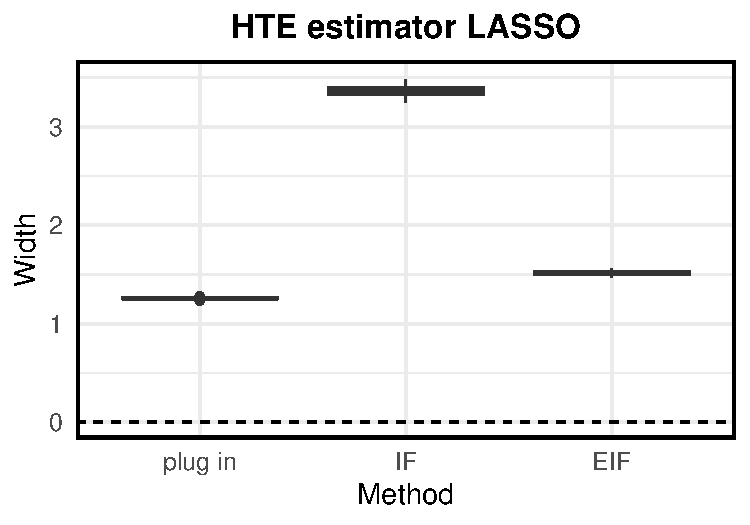
\includegraphics[clip, trim = 0cm 0cm 0cm 0cm, width = \textwidth]{plot/simulation gradient boosting CI width LASSO.pdf}
%         \end{minipage}
%         \begin{minipage}{0.3\textwidth}
%                 \centering
%                 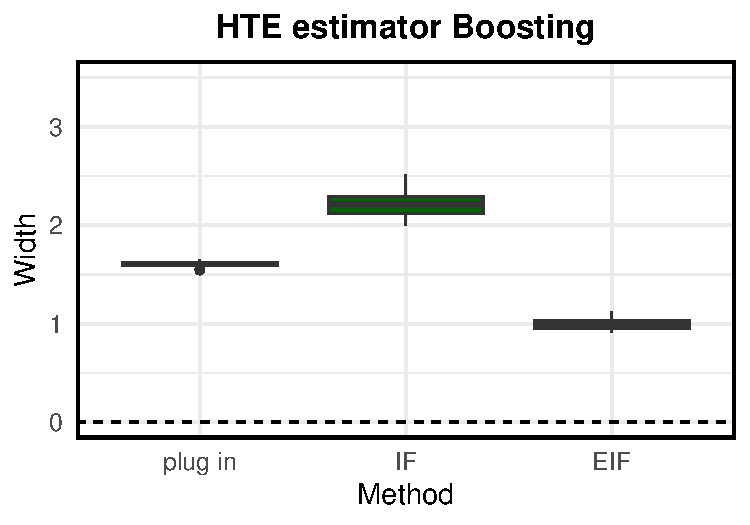
\includegraphics[clip, trim = 0cm 0cm 0cm 0cm, width = \textwidth]{plot/simulation gradient boosting CI width Boosting.pdf}
%         \end{minipage}
%         \begin{minipage}{0.3\textwidth}
%                 \centering
%                 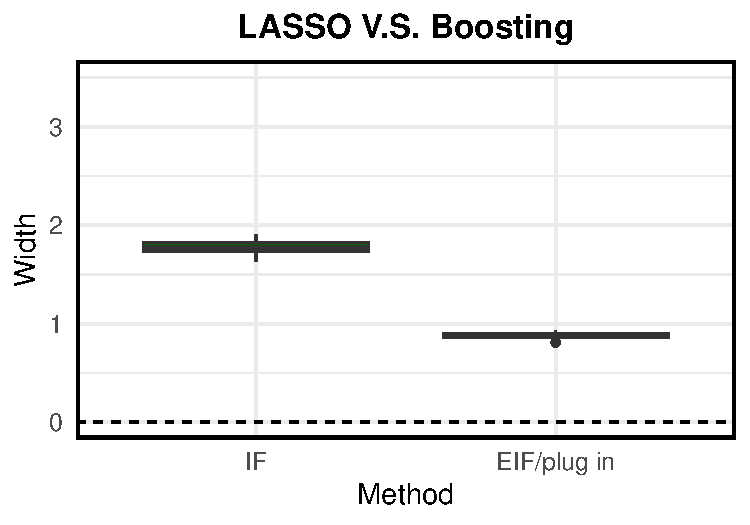
\includegraphics[clip, trim = 0cm 0cm 0cm 0cm, width = \textwidth]{plot/simulation gradient boosting CI width LASSO V.S. Boosting.pdf}
%         \end{minipage}        
%         \centering{(c) Gradient boosting with underfitting}
%          Width of the estimated absolute (LASSO, Boosting)/relative (LASSO V.S. Boosting) error's $90\%$ confidence intervals across three methods (plug in, IF, EIF) over three nuisance functions (true, estimated by linear regression, estimated by gradient boosting with underfitting).
%     \label{fig:simulation.width}
% \end{figure}


% \begin{figure}[ht]
%         \centering
%         \begin{minipage}{0.3\textwidth}
%                 \centering
%                 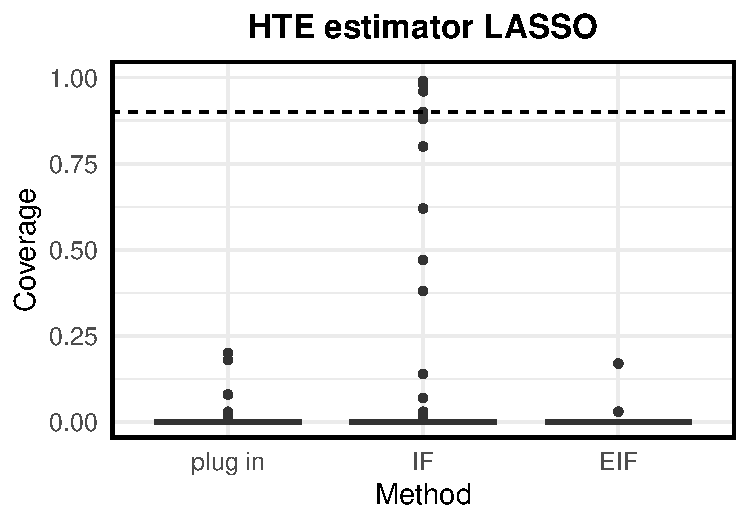
\includegraphics[clip, trim = 0cm 0cm 0cm 0cm, width = \textwidth]{plot/ACIC linear propensity linear HTE coverage LASSO.pdf}
%         \end{minipage}
%         \begin{minipage}{0.3\textwidth}
%                 \centering
%                 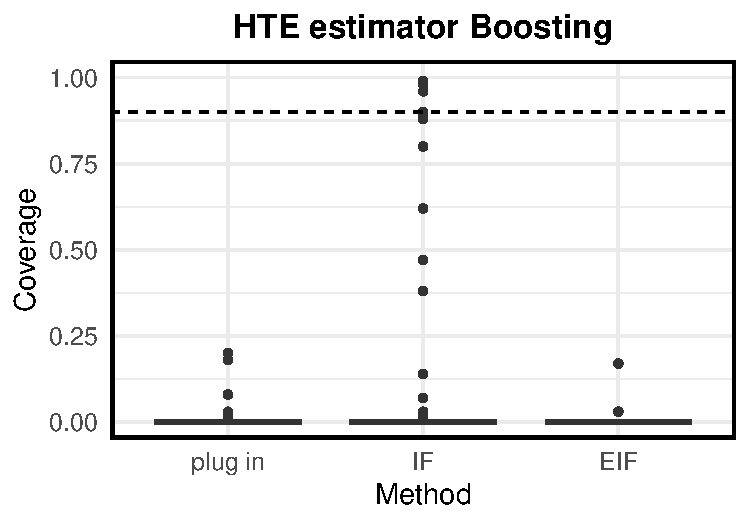
\includegraphics[clip, trim = 0cm 0cm 0cm 0cm, width = \textwidth]{plot/ACIC linear propensity linear HTE coverage Boosting.pdf}
%         \end{minipage}
%         \begin{minipage}{0.3\textwidth}
%                 \centering
%                 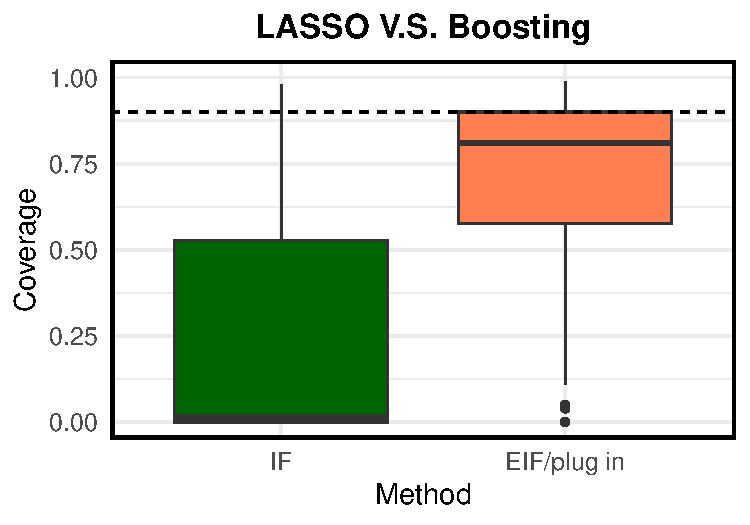
\includegraphics[clip, trim = 0cm 0cm 0cm 0cm, width = \textwidth]{plot/ACIC linear propensity linear HTE coverage LASSO V.S. Boosting.pdf}
%         \end{minipage}        
%         \centering{(a) Linear $\mu_0(x)$, $\mu_1(x)$, linear $e(x)$}
%         \begin{minipage}{0.3\textwidth}
%                 \centering
%                 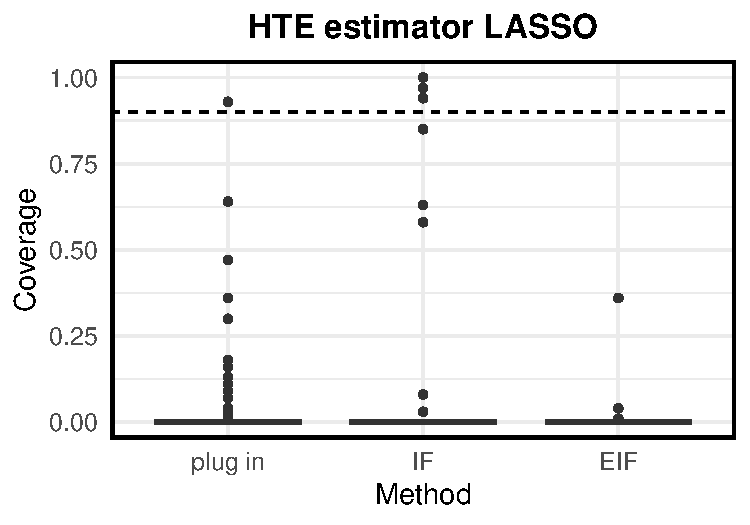
\includegraphics[clip, trim = 0cm 0cm 0cm 0cm, width = \textwidth]{plot/ACIC linear propensity nonlinear HTE coverage LASSO.pdf}
%         \end{minipage}
%         \begin{minipage}{0.3\textwidth}
%                 \centering
%                 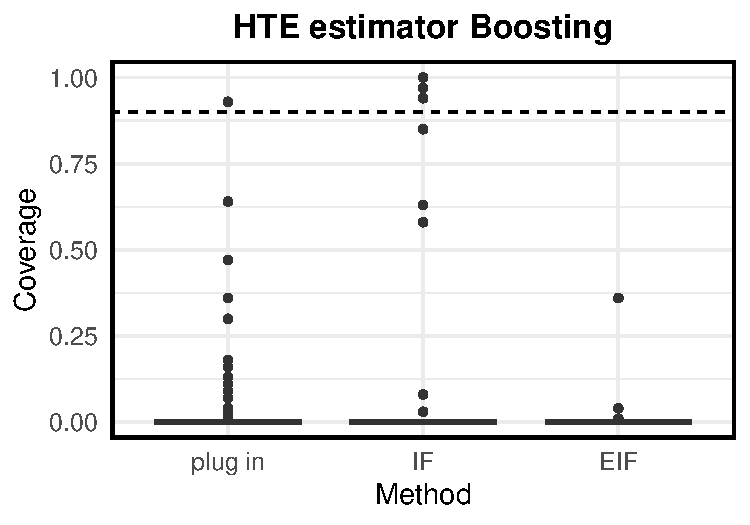
\includegraphics[clip, trim = 0cm 0cm 0cm 0cm, width = \textwidth]{plot/ACIC linear propensity nonlinear HTE coverage Boosting.pdf}
%         \end{minipage}
%         \begin{minipage}{0.3\textwidth}
%                 \centering
%                 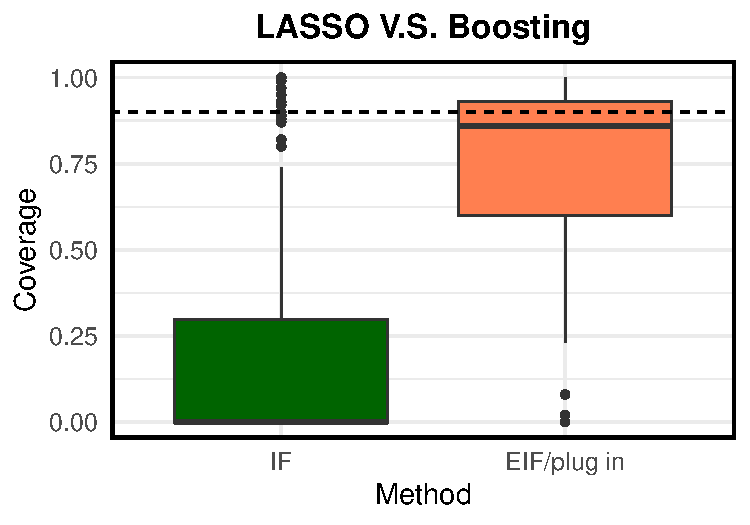
\includegraphics[clip, trim = 0cm 0cm 0cm 0cm, width = \textwidth]{plot/ACIC linear propensity nonlinear HTE coverage LASSO V.S. Boosting.pdf}
%         \end{minipage}        
%         \centering{(b) Nonlinear $\mu_0(x)$, $\mu_1(x)$, linear $e(x)$}  
        
%         \begin{minipage}{0.3\textwidth}
%                 \centering
%                 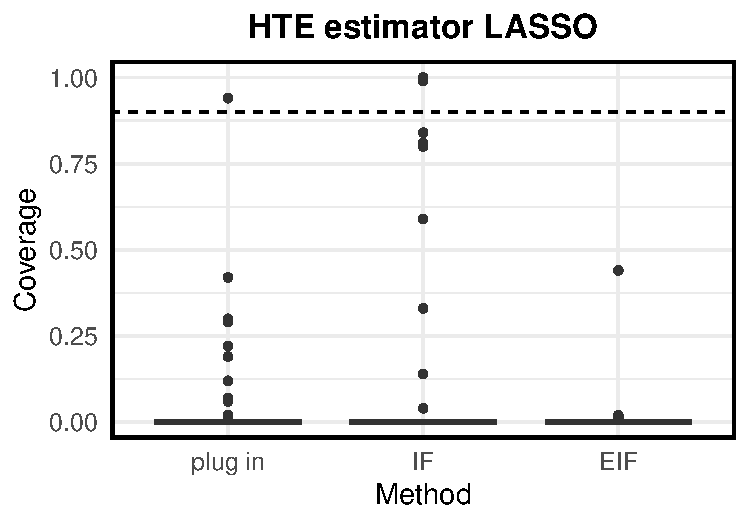
\includegraphics[clip, trim = 0cm 0cm 0cm 0cm, width = \textwidth]{plot/ACIC nonlinear propensity linear HTE coverage LASSO.pdf}
%         \end{minipage}
%         \begin{minipage}{0.3\textwidth}
%                 \centering
%                 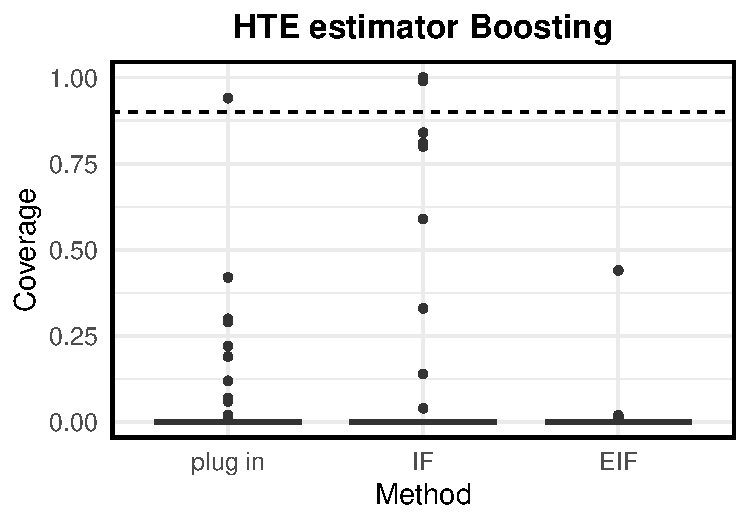
\includegraphics[clip, trim = 0cm 0cm 0cm 0cm, width = \textwidth]{plot/ACIC nonlinear propensity linear HTE coverage Boosting.pdf}
%         \end{minipage}
%         \begin{minipage}{0.3\textwidth}
%                 \centering
%                 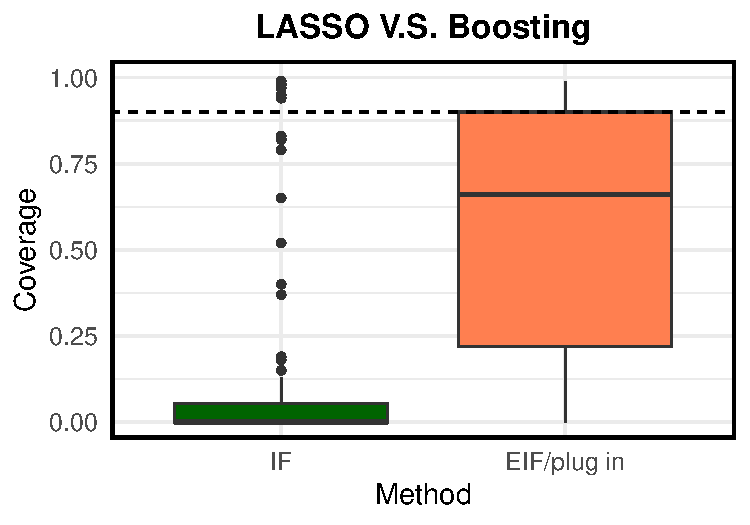
\includegraphics[clip, trim = 0cm 0cm 0cm 0cm, width = \textwidth]{plot/ACIC nonlinear propensity linear HTE coverage LASSO V.S. Boosting.pdf}
%         \end{minipage}        
%         \centering{(c) Linear $\mu_0(x)$, $\mu_1(x)$, nonlinear $e(x)$}      
%         \begin{minipage}{0.3\textwidth}
%                 \centering
%                 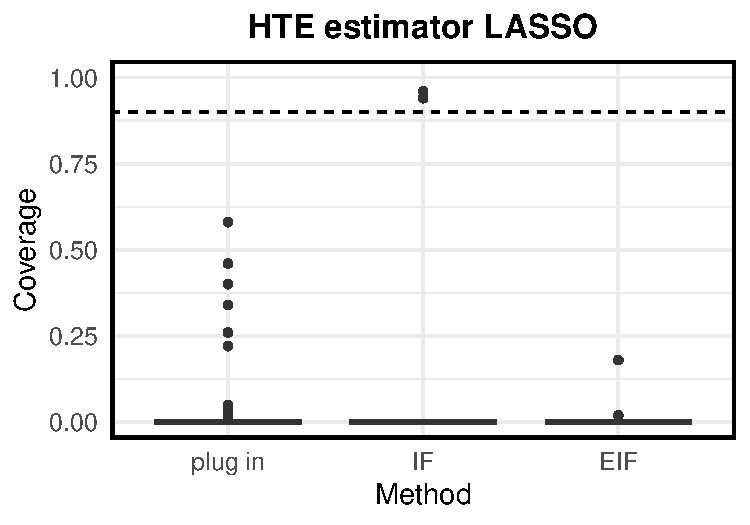
\includegraphics[clip, trim = 0cm 0cm 0cm 0cm, width = \textwidth]{plot/ACIC nonlinear propensity nonlinear HTE coverage LASSO.pdf}
%         \end{minipage}
%         \begin{minipage}{0.3\textwidth}
%                 \centering
%                 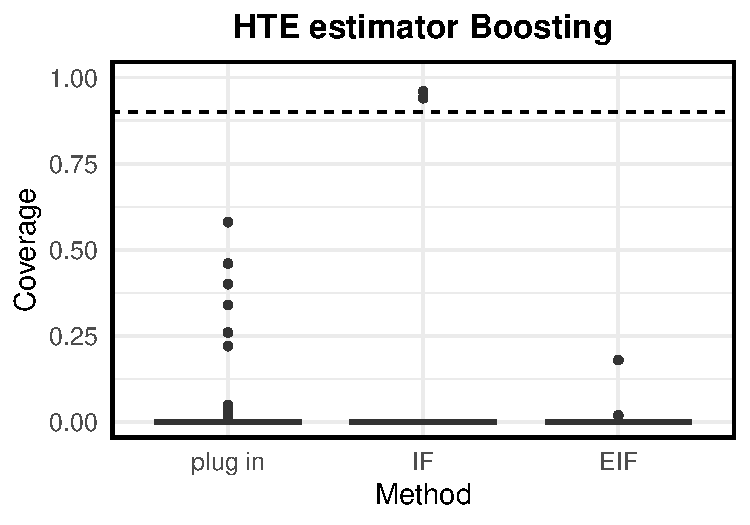
\includegraphics[clip, trim = 0cm 0cm 0cm 0cm, width = \textwidth]{plot/ACIC nonlinear propensity nonlinear HTE coverage Boosting.pdf}
%         \end{minipage}
%         \begin{minipage}{0.3\textwidth}
%                 \centering
%                 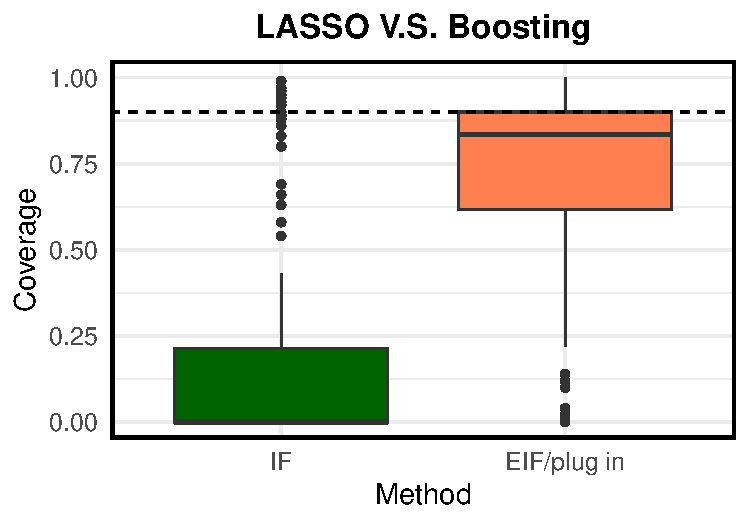
\includegraphics[clip, trim = 0cm 0cm 0cm 0cm, width = \textwidth]{plot/ACIC nonlinear propensity nonlinear HTE coverage LASSO V.S. Boosting.pdf}
%         \end{minipage}        
%         \centering{(d) Nonlinear $\mu_0(x)$, $\mu_1(x)$, nonlinear $e(x)$} 
%         \caption{
%         Coverage of the estimated absolute (LASSO, Boosting)/relative (LASSO V.S. Boosting) error's $90\%$ confidence intervals across three methods (plug in, IF, EIF) over four scenarios of the ACIC competition data ((a) to (d)).   
%         }
%     \label{fig:ACIC.coverage}
% \end{figure}



% \end{document}
